\documentclass[12pt]{article}
\usepackage[margin=1in]{geometry}
\usepackage[utf8]{inputenc}
\usepackage{tocloft}
\usepackage{color}
\usepackage{graphicx}
\usepackage{setspace}
\usepackage{subcaption}
\usepackage{wrapfig}
\usepackage{hyperref}
\usepackage{amsmath}
\graphicspath{{./figs/}}
\newcommand{\comment}[1]{\textcolor{red}{{\tt #1}}}
\newcommand{\nij}[1]{\textcolor{blue}{{\tt #1}}}
\newcommand{\todo}[1]{\textcolor{magenta}{TO DO: {\tt #1}}}

%% For text that you would like someone to improve.
\newcommand{\weak}[1]{\textcolor{green}{{\it #1}}}


\begin{document}
\pagenumbering{gobble}
%% Title Page
\begin{center}
    {\Large Image Similarity Tools to Combat Human Trafficking}\\
    {\Small Dissertation Proposal}
    %% Other title ideas:
    % Explainable AI for Image Analysis to Combat Human Trafficking
    % Image Analysis to Combat Human Trafficking Using an Investigative Approach
    % Investigative AI: An Object-Centric Approach for Image Analysis to Combat Human Trafficking
    % Fighting Human Trafficking Using Image Analysis
    
    
    \vspace{1.5in}
        \begin{tabular}{|l|l|}
        \hline
        PhD Candidate    & Abigail Stylianou\\
        \hline
        Date & August 8, 2018 \\
        \hline
        Committee Members & Sanmay Das, Ph.D. (Committee Chair \& Advisor) \\
            & Tao Ju, Ph.D. \\
            & Ayan Chakrabarti, Ph.D. \\
            & Alvitta Ottley, Ph.D. \\
            & Robert Pless, Ph.D. \\
            & Richard Souvenir, D.Sc. \\
            \hline
        \end{tabular}
\end{center}
\newpage

%% Table of Contents
\thispagestyle{empty}
\setcounter{tocdepth}{3}
\tableofcontents
\newpage
\thispagestyle{empty}
\listoffigures
\newpage

\doublespacing
\pagenumbering{arabic}
\setcounter{page}{1}

Images often play a significant role in investigations of human trafficking. Traffickers share photographs of their victims among criminal networks and  post them in online advertisements. Such images often contain clues as to
the location where the image was captured. In the course of a criminal investigation, determining where a victim was photographed can be useful to, for example, learn if the victim was moved across state lines or if particular locations serve as ``hot spots'' where victims might be trafficked again. Much of this photographic evidence is captured in hotel rooms~\cite{stltodayHotels}.

The focus on my doctoral research has been on building novel datasets, algorithms and systems that support determining where these photographs were taken. To support this, we have developed a system called TraffickCam, which consists of a massive database of hotel room photographs and a machine learning-based image search system for law enforcement to compare victim photographs to the photographs in that database. The database of hotel room photographs contains several million hotel room images collected from both publicly available travel websites (e.g., Expedia, TripAdvisor) and the over 100,000 users of our mobile application that allows travelers to submit images of hotel rooms they visit~\cite{aipr2015}. TraffickCam uses neural networks to support image-based search for members of law enforcement. Images containing victims of trafficking in hotel rooms are provided as input, and the system returns the hotels with the most similar images~\cite{aipr2017}.

TraffickCam is presently being used by our law enforcement collaborators in the St. Louis County Police Department and the National Center for Missing and Exploited Children. While the consensus is that the system we have developed through our research and work to date is a significant improvement over their current, manual investigative process, these collaborators have highlighted ways that the existing image-based search could better align with their investigative approaches. First, they often would like to be able to search with a smaller part of the victim photograph, such as a particular object that seems unique. Second, they want easy to understand explanations of why the AI-system returned a specific result, both to increase their understanding of the results and to potentially be used as evidence when securing search warrants at particular hotel locations. Implementing these desired capabilities is non-trivial and not supported at scale by existing work in computer vision and machine learning.

In this proposal, I will discuss the research and work I have already done and that I intend to do in the remaining course of my doctoral research in order to support these desired capabilities and to provide a more useful computer vision and machine learning-based investigative tool to investigators of human trafficking.

\section{Related Work}

Extracting real-world context from images is a fundamental goal in the field of computer vision. The proposed work in my dissertation cross-cuts numerous problems in computer vision, such as scene recognition, image geolocation, object segmentation, and object recognition. Each of these areas has significant history; in this review, I focus on methods most related to our problem.

\paragraph{Scene Recognition and Image Geolocation}
Recognizing the scene from which an image was captured has been a problem of great interest in the computer vision community. One line of work focuses on the problem of identifying the scene category (e.g., park, beach, parking lot) rather than particular locations. Recently, there has been increased interest in estimating the geographic location at which an image was captured based on its
appearance~\cite{baatz2012large,doersch2012what,hays2008im2gps,knopp2010avoiding,li2009landmark,zhou2014recognizing}. These approaches rely on visual cues such as sun
position~\cite{cozman1995robot,lalonde2010sun,workman2014rainbow}, shadows~\cite{junejo2010gps,sandnes2011determining,wu2010geo}, and weather~\cite{jacobs11geolocate,jacobs08geoorient,sunkavalli2008color}. Alternatively, the localization problem can be formulated as an image retrieval task where publicly-available geotagged images serve as a database, and, given a query image,  its location is inferred by finding visually similar images in the dataset~\cite{baatz2012large,chen2011city,crandall2009mapping,hays2008im2gps,jacobs07geolocate,schindler2007city,torii2013visual,zamir2010accurate,zhou2014recognizing}. While these approaches work well for outdoor scenes and/or unique landmarks, they are not well-suited to the problem of discriminating between similar-looking indoor scenes, such as hotel rooms.

\paragraph{Object Segmentation and Identification} Scenes can often be decomposed into a collection of objects. Identifying objects in a scene is another task with a long history in computer vision. Similar to scene recognition, the goal is to classify new instances as belonging to one of a pre-defined set of known classes. For objects, there is the additional challenge of locating which pixels of an image correspond to the object. Modern object detectors~\cite{DBLP:journals/corr/LiuAESR15,yolov3,DBLP:journals/corr/RenHG015} combine both of these tasks. These methods are useful for identifying the types of objects typically found in images of hotel rooms, such as beds, TVs, and lamps. Additionally, object detectors are readily available as off-the-shelf tools that can be applied to new images. However, identifying the objects in a scene is only one step in the process, and not sufficient for the larger problem of hotel room identification. Additionally, as we demonstrate in Section~\ref{sec:usability}, modern general-purpose object detectors do not perform well on the types of images collected for our problem.

\paragraph{Visualizing Neural Networks} Visualizations provide a way to better understand the learning process underlying deep neural networks. Much of the work in this area focuses on visualizations for classification networks (networks that provide a class label for an image) and not similarity networks (networks that produce similar output feature vectors for images from the same class; these are the types of networks that support TraffickCam). While networks used for each type of problem share many similarities, the differences in the output (i.e., sparse vs. dense feature vectors) is significant, requiring new methods for visualizing similarity networks. Previous work on visualizing convolutional neural networks can be broadly categorized by the depth of the portion of the networked being visualized. Some methods provide visualizations that highlight the inner layer activations~\cite{netdissect2017,visualization_techreport,scenecnn_iclr15}. A majority of the work targets the output layer to produce visualizations which seek to explain why classification networks output a particular label for an image. These include approaches that mask off parts of the input images and provide a visual quantification of the impact on the output classification~\cite{ZeilerF13}. Another approach generates saliency maps, which represent which pixels in an image contributed to a particular output node~\cite{deepInside}. There has been work that generates class activation maps, which map an output back to the last convolutional layer in the network by weighting the filters in that layer by the weights between the final pooling layer and the output feature~\cite{cam}. Inception~\cite{szegedy2015going}, which hallucinates images that activate a particular class from random noise, can also serve as visualization tool to provide insight into the learning process. 

Much of the work in similarity learning with deep neural networks focuses on learning better similarity functions using, for example, pairwise losses~\cite{sun2014deep,wang2014learning,yi2014deep}, triplet losses~\cite{HermansBeyer2017Arxiv,schroff2015facenet,song2016deep,ustinova2016learning}, and direct embedding~\cite{Proxy}. Compared to the efforts toward understanding classification networks, there has been much less work in visualizing and analyzing similarity networks. One method visualizes the similarity of single filters from the different convolutional layers of an embedding network~\cite{Ahmed_2015_CVPR}. Another method computes image similarity as the inner product between the normalized elements of a final max pooling layer and produces a visualization with bounding boxes around highly active regions for the ten features that contribute most to the similarity of a pair of images~\cite{RTC16,tolias2016rmac}. 

\paragraph{AI for Fighting Human Trafficking}
There have been some efforts to apply machine learning, computer vision, and natural language processing to fight human trafficking. Most of the computer vision-based approaches focus on the optical character recognition on the text content of online advertisements, such as phone numbers and descriptions of the location. A number of methods build models from the extracted data in order to support law-enforcement facing search engines~\cite{alvari2017semi,dubrawski2015leveraging,kejriwal2017investigative,szekely2015building}. Other approaches focus on integrating text and images~\cite{tong2017combating} using a deep learning model in an attempt to discern whether an online advertisement includes a victim of trafficking. There are also some larger-scale projects, such as Thorn\footnote{\url{https://www.wearethorn.org/}}, which incorporate computer vision-based methods, including facial re-identification, as part of a larger effort toward addressing child sex trafficking and sexual abuse.

\section{Current Gaps in Data, Research, and Knowledge}
\label{sec:gaps}

The design of usable computer vision-based software for non-experts, such as human trafficking investigators, introduces a number of challenges. In the course of my dissertation work, I will be focused on how to build computer vision-based software tools that are accessible for non-experts, and specifically for law enforcement investigators of human trafficking. This work will require exploring some existing gaps in usability and explainability in computer vision and machine learning-based image search systems. First, there is a usability gap between law enforcement and software tools: the types of searches that are most useful to an investigator may not be supported by the software tools. Second, there is an explainability gap between the investigator and the AI algorithms that support the software tools: an investigator may not understand why the algorithms returned a particular result.

\subsection{Opportunities to Improve Usability}
One of our law enforcement collaborators, an investigator with the Saint Louis County Police Department, has tried in the past to use software to analyze images of trafficked victims in hotel rooms. He would submit photographs to Google Image Search hoping to find similar images from the same hotel. This process would rarely produce useful results. The investigator would then revert to using human intelligence, asking others if they recognized the hotel in the photograph. The reason that general-purpose automated image search platforms such as Google Image Search provide unsatisfactory results for this task is because they are trained for a more generic version of finding ``similar images'', rather than for the task of recognizing a hotel, and, in order to achieve the scale of searching across all images that Google indexes, they learn a single, small descriptor of the whole image.  For our problem, a search that is based on the similarity of single descriptors for whole images is problematic both because the victim often takes up a significant percentage of the pixels in the query image and, especially in hotels, similar visual appearance may not correspond similar location and vice-versa (e.g., the same headboard in different hotels, or different colored bed linens in the same hotel). Currently available software tools and vision algorithms are not designed to address this type of task. 

In the manual analysis of images, investigators often focus on particular objects in the scene, specifically those that are interesting or anomalous, rather than considering the image as a whole. This suggests an object-centric approach to automated methods for image matching. Figure~\ref{fig:wholeImVsObjectCentric} demonstrates the difference between a standard image-based search that considers whole images with our proposed object-centric approach, where the investigator highlights a specific object in the image, and the search returns images containing similar looking objects. In Figure~\ref{fig:wholeImage}, the original search approach finds images with similar furniture configurations and color profiles. In the object-centric approach in Figure~\ref{fig:objectCentric}, the investigator highlighted the yellow lamp, and the search returns other images that contain similar lamps, regardless of the other content in the room. This proposed object-specific approach is not supported by existing approaches to image-based search

\begin{figure}
    \centering
    \begin{subfigure}[b]{3.2in}
        \begin{subfigure}[b]{1.05in}
            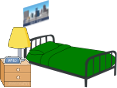
\includegraphics[height=.77in]{figs/cartoonQueries/wholeIm1.png}
        \end{subfigure}
        \unskip \vrule
        \begin{subfigure}[b]{2.1in}
            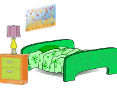
\includegraphics[height=.77in]{figs/cartoonQueries/wholeIm2.png}
            
\includegraphics[height=.77in]{figs/cartoonQueries/wholeIm3.png}
        \end{subfigure}
        \caption{Whole Image Search}
        \label{fig:wholeImage}
    \end{subfigure}
    \begin{subfigure}[b]{3.2in}
        \begin{subfigure}[b]{1.05in}
            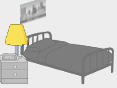
\includegraphics[height=.77in]{figs/cartoonQueries/justLamp1.png}
        \end{subfigure}
        \unskip \vrule
        \begin{subfigure}[b]{2.1in}
            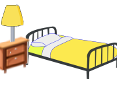
\includegraphics[height=.77in]{figs/cartoonQueries/justLamp2.png}
            
\includegraphics[height=.77in]{figs/cartoonQueries/justLamp3.png}
        \end{subfigure}
        \caption{Object-centric Image Search}
        \label{fig:objectCentric}
    \end{subfigure}
    \caption[Whole image search vs. object-centric search]{(a) In a typical image search based on the whole image the results are the images that look most similar to the entire image (e.g., similar color profiles and furniture in the same configuration). (b) In our object-centric image search, the input is a selected object of interest, and the results are images that contain objects that are most similar to the query object (e.g., images with yellow lamps).}
    \label{fig:wholeImVsObjectCentric}
\end{figure}

\subsection{Opportunities to Improve Explainability}
Even outside of the domain of software tools for law enforcement, explainability is a major concern in the field of Artificial Intelligence. In fact, some countries have enacted or are proposing laws to ensure that AI algorithms used to make decisions are explainable and/or provide evidence for the resulting prediction~\cite{eu_regulations}.
\begin{wrapfigure}{r}{3in}
\centering
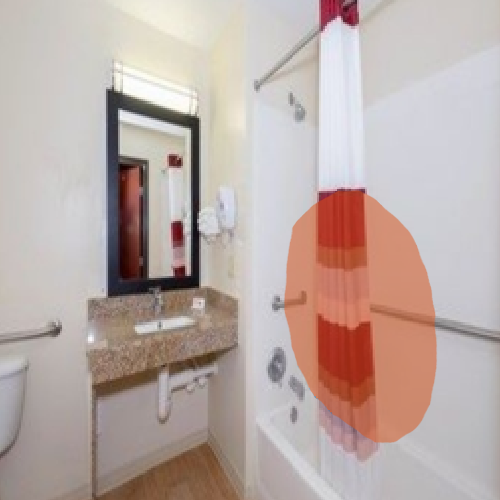
\includegraphics[width=1.4in]{vis/vis_im1}
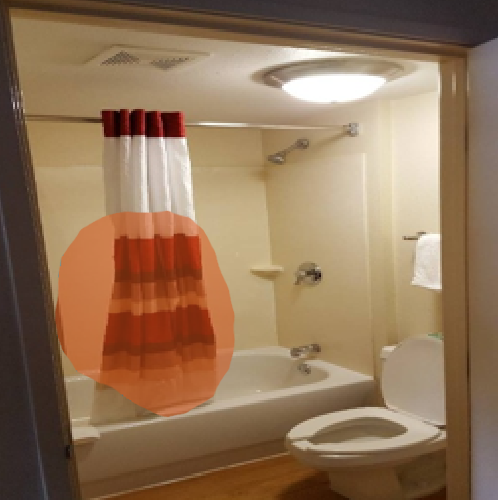
\includegraphics[width=1.4in]{vis/vis_im2}
\caption[Example of object matching search]{An example visualization where the system matched the images based on the shower curtains, even though other components of the scene are dissimilar.}
\label{fig:exampleObjHighlighting}
\end{wrapfigure}
In the context of our problem, this relates to the search results returned for a particular query. An investigator may want to understand why particular images did or did not show up among the top results. One approach to providing explainability is via data visualizations, where image regions of the search results that contributed the most to the prediction are highlighted, as depicted in Figure~\ref{fig:exampleObjHighlighting}.

\section{Research Questions}
The purpose of the work set out in the dissertation proposal is to perform the fundamental research needed to make image search more effective in investigations of human trafficking.  This research includes creating new algorithms to allow investigators to perform object-specific image queries, building new visualization tools, and integrating these developments in a system that is shared with law enforcement for both actual use and ongoing feedback. This proposal includes three specific research questions:

\begin{itemize}
    \setlength\itemsep{.1em}
    \item \emph{How can large scale visual search be specialized to the problem of recognizing hotels?}\\
    We have developed and deployed a large scale system for human trafficking investigators to determine which hotels victims were photographed in. This system is currently being tested by human trafficking investigators around the country.
    \item \emph{What is the best image representation to support exploratory investigative search?} \\
    I intend to create approaches for object-centric image analysis in the context of search over millions of images, focusing on identifying images that have the same objects that appear in a query image.
    \item \emph{How can convolutional neural networks that produce embeddings be visualized to understand why images are similar?} \\
    For large scale image search based on the similarity of the features output from a convolutional neural network, we will develop visualization approaches that explain why a result image is similar to a query image. These visualizations will provide intuition for human trafficking experts on what parts of the images the network focuses on, and why a particular query may or may not have been successful.
\end{itemize}

My objective is to substantially improve the effectiveness of image search in investigations of human trafficking.  These objectives will be measured at the level of improved image search accuracy on standard and new datasets, and by integrating the advances into an existing TraffickCam image search interface and soliciting feedback on the effectiveness of the search tools from real law enforcement users.

\section{TraffickCam}
\begin{figure}
    \centering
    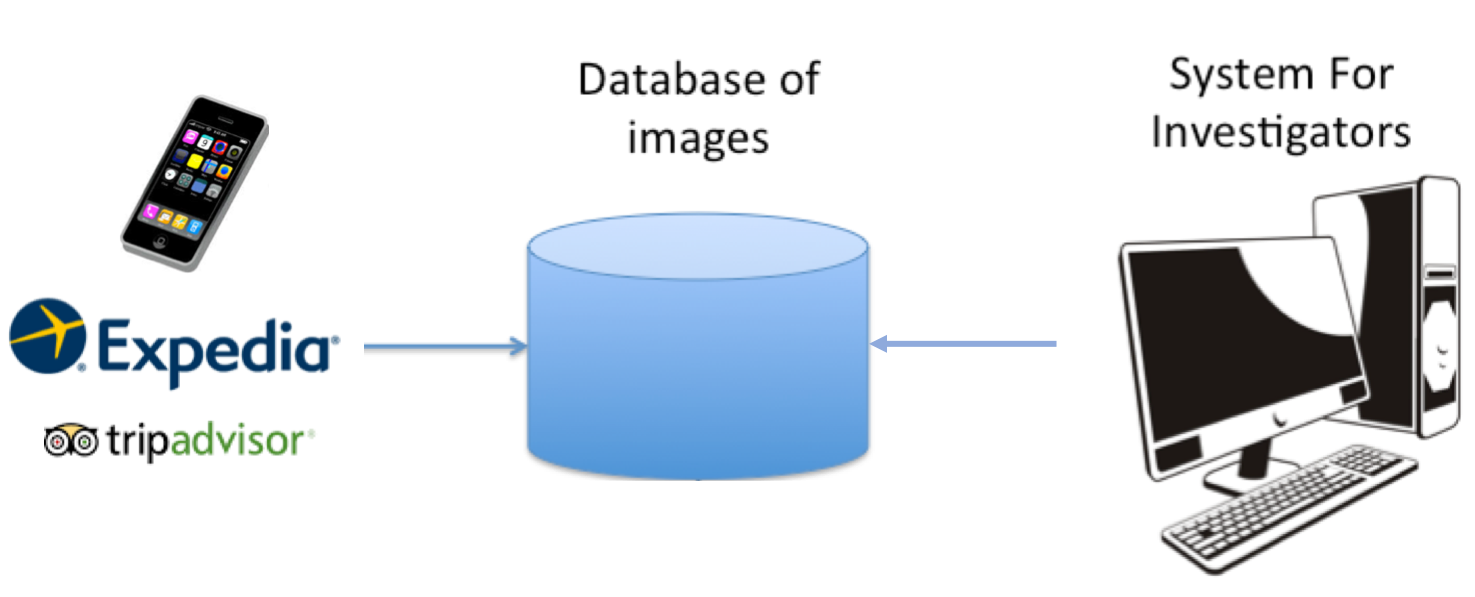
\includegraphics[width=.85\textwidth]{figs/tcOverview/tcWorkflow.png}
    \caption[TraffickCam overview]{A database of carefully annotated pictures of hotel rooms offers an important investigative tool.  TraffickCam combines a crowd-sourcing mobile phone app that collects images from travelers with existing publicly available images of hotels into a massive database of hotel room photographs. We then extract features from a neural network trained on recognizing hotel rooms for each image and provide provisioned members of law enforcement an interface to  match images of victims in hotel rooms to similar images in the database.}
    \label{fig:tcam}
\end{figure}

The research that I will perform over the remainder of my dissertation builds upon the ongoing efforts to develop TraffickCam, a system designed for law enforcement to analyze photographs of victims of human trafficking. TraffickCam consists of a large dataset of hotel room images and a computer vision-based image search platform to help investigators determine the hotel where the victim was photographed. Early versions of TraffickCam have been tested by our collaborators in law enforcement, who provide a willing user base motivated to test the new approaches developed over the remaining course of my dissertation. In this section I describe the components and current capabilities of TraffickCam, and the research and work completed to date to make it a functional image search tool for human trafficking investigators.

\subsection{Data Collection}

\begin{wrapfigure}{r}{2.5in}
    \centering
    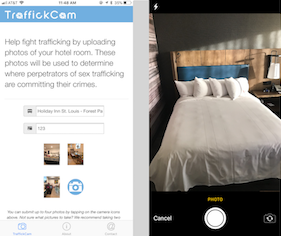
\includegraphics[width=2.4in]{figs/appScreenshotsCrop.png}
    \caption{Screenshots of the TraffickCam iOS application}
    \label{fig:tcamScreenshots}
\end{wrapfigure}

TraffickCam frames the investigative task of identifying where a trafficking victim was photographed as an image similarity problem, where the goal is to find the most similar images to a query in a database of images. To support this large-scale image similarity challenge, we train a convolutional neural network to learn an image similarity function for hotel room images. This is the same technology that has fueled other automated computer vision algorithms to achieve near human-level performance for identification and recognition. This technology has formed the basis for applications that can identify landmarks and tourist attractions using a mobile device, identify shoes and clothing and provide recommendations for fashionable matching items, and automatically translate text captured in images and videos in real time. 

For all of these problems, including ours, training these models requires huge volumes of image data. To support this, we have created a database of 2.8 million photographs of hotel rooms from over 250,000 hotels around the world. These photographs are collected from both publicly available sources of travel photographs, such as those on travel websites like Expedia and TripAdvisor, and also through the TraffickCam smartphone application, which allows travelers to submit photographs of their hotel rooms to support investigations of human trafficking. Screenshots of the TraffickCam iOS application are shown in Figure~\ref{fig:tcamScreenshots}. Travelers select their hotel from a list of nearby hotels, enter their room number and provide images of different views of their hotel room. The TraffickCam application has over 100,000 users on Android and iOS devices, and hundreds of new photographs are uploaded to the database every day.

\subsection{Training a Neural Network to Match Hotel Room Images}
\label{sec:training}

The initial approach for implementing the back-end for TraffickCam followed recent work in computer vision and machine learning by training a convolutional neural network to convert images into meaningful feature representations (small numerical descriptors of the image). Specifically, we used TensorFlow to train the Resnet-50 convolutional neural network architecture~\cite{resnet}, using the version of margin-based triplet loss described in~\cite{HermansBeyer2017Arxiv}. This approach encourages the neural network to learn a model where the feature representations extracted from images of the same hotel are similar to each other, but different from the feature representations extracted from images at different hotels. The problem of hotel identification in the human trafficking context presents some unique challenges in performing this training.

\begin{figure}
    \centering
    \begin{subfigure}[b]{2.55in}
    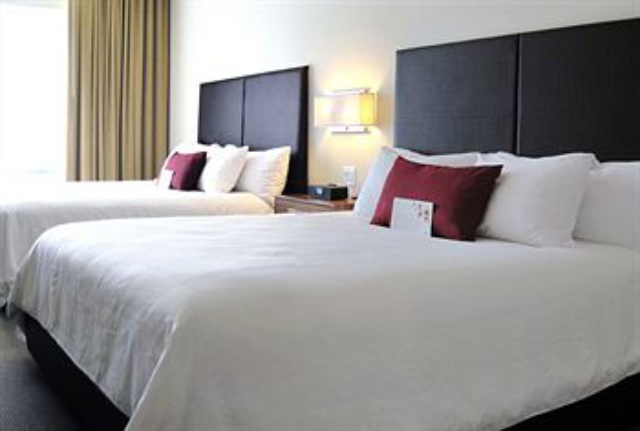
\includegraphics[height=1in]{figs/exampleDbIms/expedia1.jpg}
    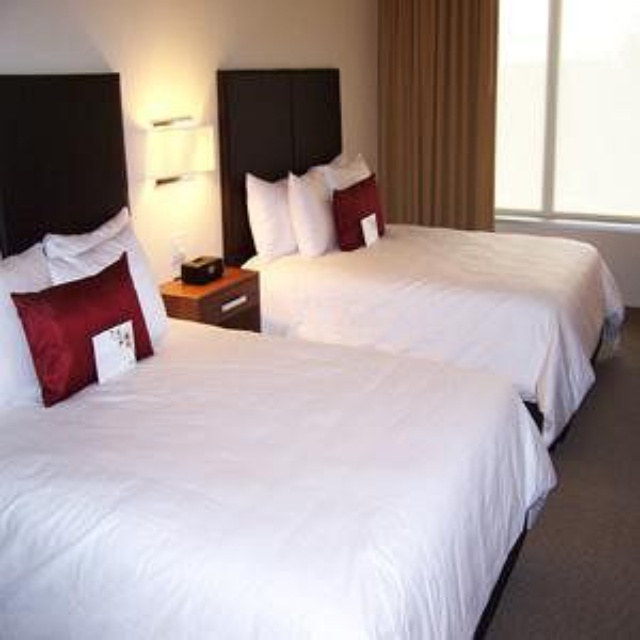
\includegraphics[height=1in]{figs/exampleDbIms/expedia2.jpg}
    \caption{Web images}
    \end{subfigure}
   \begin{subfigure}[b]{2.65in}
    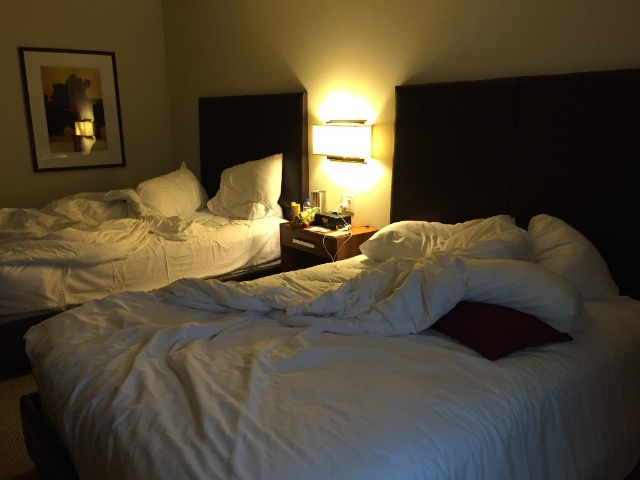
\includegraphics[height=1in]{figs/exampleDbIms/tc1}
    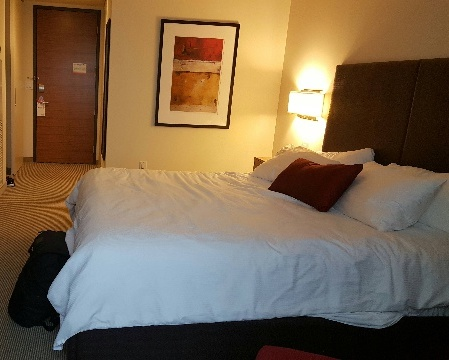
\includegraphics[height=1in]{figs/exampleDbIms/tc2}
    \caption{App images}
    \end{subfigure}
   \begin{subfigure}[b]{1.2in}
    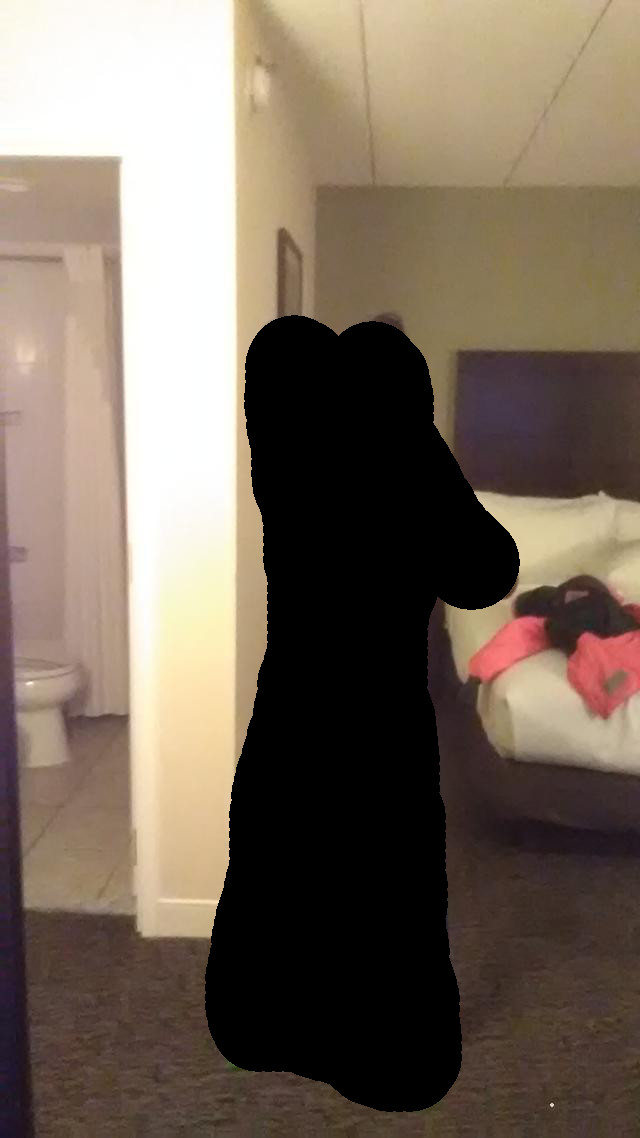
\includegraphics[height=1in]{figs/exampleDbIms/backpage1.jpg}
    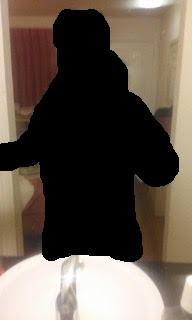
\includegraphics[height=1in]{figs/exampleDbIms/backpage2.jpg}
    \caption{Query images}
    \end{subfigure}
    \caption[Image variability from different sources]{Examples images from (a) hotel websites, (b) the TraffickCam crowdsourcing app, and (c) queries used by law enforcement. The images in (a) and (b) are from the same hotel, highlighting the significant differences in the properties of images from different sources.}
    \label{fig:domainImages}
\end{figure}

The biggest challenge is known as the problem of domain adaptation. While, to date, our database of hotel room images contains millions of Internet images and hundreds of thousands images crowdsourced from the mobile app, these images can be quite different from each other, and even more different from the types of images used as queries by law enforcement. The publicly available travel photographs images are abundant and useful for discriminating between hotel rooms, but these scenes are often lit artificially and professionally captured, and the resulting images are visually dissimilar from the types of images used in human trafficking advertisements (i.e., captured by amateurs using cell phone cameras). The opposite is true for the images from the mobile app users: they share visual characteristics with the query images, but are far less abundant and sometimes uninformative due to the lighting or portion of the scene captured. Figure~\ref{fig:domainImages} shows sample images from each of these different sources.

TraffickCam incorporates a number of modifications to the normal training process to address domain adaptation. (1)~The training set only contains examples from hotels that have both images from travel websites and images from our mobile application. This insures that the neural network is exposed to large variability among images and forced to map these images to similar feature representations. (2)~During training, the images are modified to imitate the properties observed in the real victim photographs. The images are pre-processed to include people-shaped masks over portions of the images, by applying lighting and color filters similar to those used on social media, and by rotating and cropping the images.

Figure~\ref{fig:topKaccuracy} shows a comparison between neural networks trained on the TraffickCam dataset, the TraffickCam dataset with the data augmentation techniques described above, and two pre-trained networks used for image search, trained on the ILSVRC~\cite{ILSVRC15} and Places-365~\cite{zhou2017places} datasets, respectively.

\begin{wrapfigure}{r}{3.2in}
    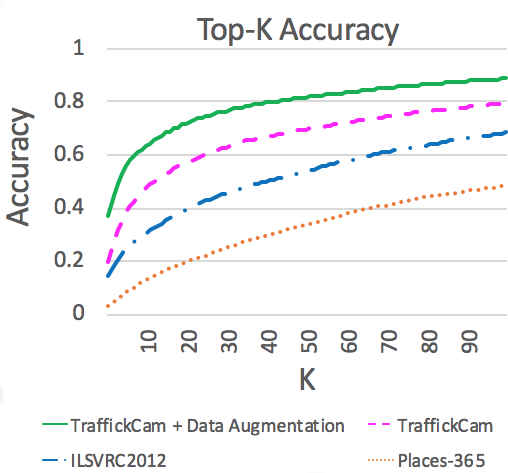
\includegraphics[width=3.1in]{figs/top-k.png}
    \caption[Accuracy of current TraffickCam search]{Comparison of TraffickCam and related neural network approaches. Top-K accuracy is the percentage of results where a correct match was within the top K matches.}
    \label{fig:topKaccuracy}
\end{wrapfigure}
For this experiment, we create a query set of images from a subset of the crowdsourced images, so the hotel is known. While images from the query set are included in the database, no images from any hotel in the query set are used for training the models. A result is considered a match if the database image comes from the same hotel. The TraffickCam search using data augmentation techniques outperforms the next best method non-TraffickCam network by $\sim$22\% in Top-1 accuracy (i.e., matching the correct hotel with the first result). The combination of the hotel data and training modifications allow TraffickCam to outperform the other approaches at the task of identifying hotel rooms from occluded, blurry, or otherwise modified query images.

\subsection{Real-World Queries with TraffickCam}

Recall that investigators currently try to use Google Image Search for this image matching task. Figure~\ref{fig:tcamResults} shows a comparison between TraffickCam and Google Image Search on a real world query where a victim occludes a large amount of the image. In this case, the query was known to be from a Chicago Marriott hotel. The top five results from TraffickCam are from the exact hotel or another Marriott hotel, containing the same artwork and headboard. By comparison, Google Image Search provides seemingly nonsensical results, likely due to the large masked off portion of the image where the victim is located.

\begin{figure}
    \centering
    \begin{subfigure}[b]{1.6in}
        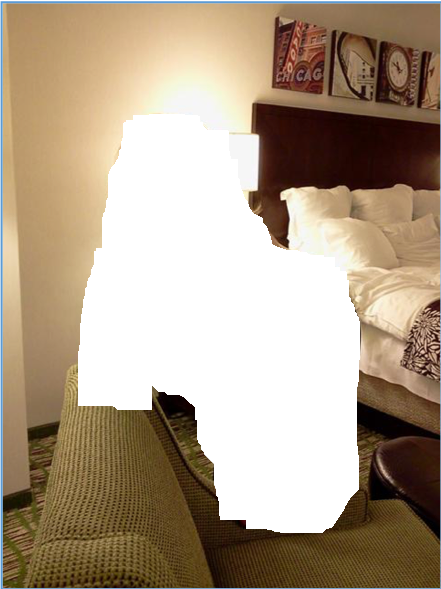
\includegraphics[width=1.5in]{figs/exampleSearch/masked.png}
        \caption{Query}
        \label{fig:tcamResults_query}
    \end{subfigure}
    \unskip \vrule \hspace{0pt}
    \begin{subfigure}[b]{4.5in}
        \begin{subfigure}[b]{4.4in}
            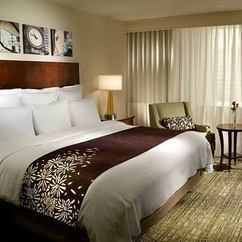
\includegraphics[width=.85in]{figs/exampleSearch/1}
            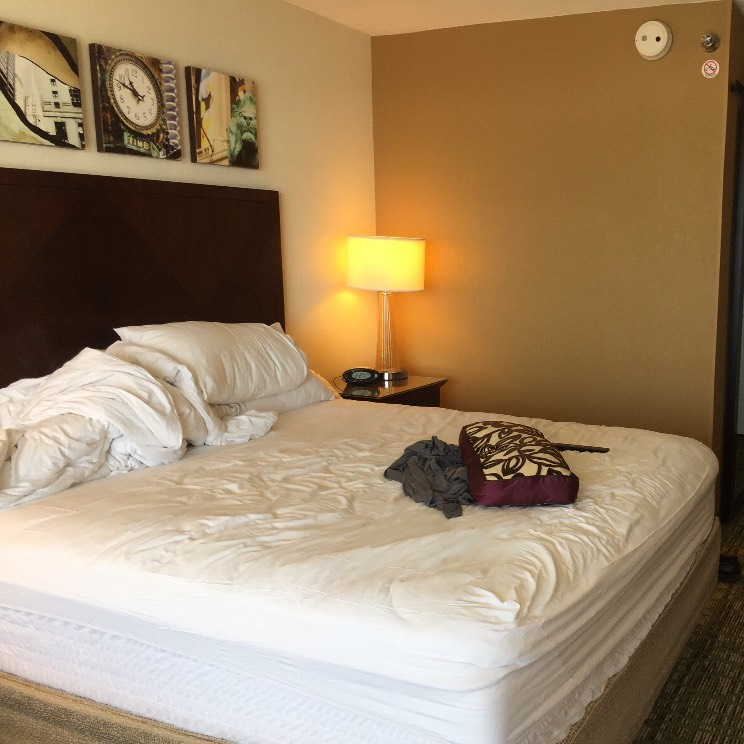
\includegraphics[width=.85in]{figs/exampleSearch/2}
            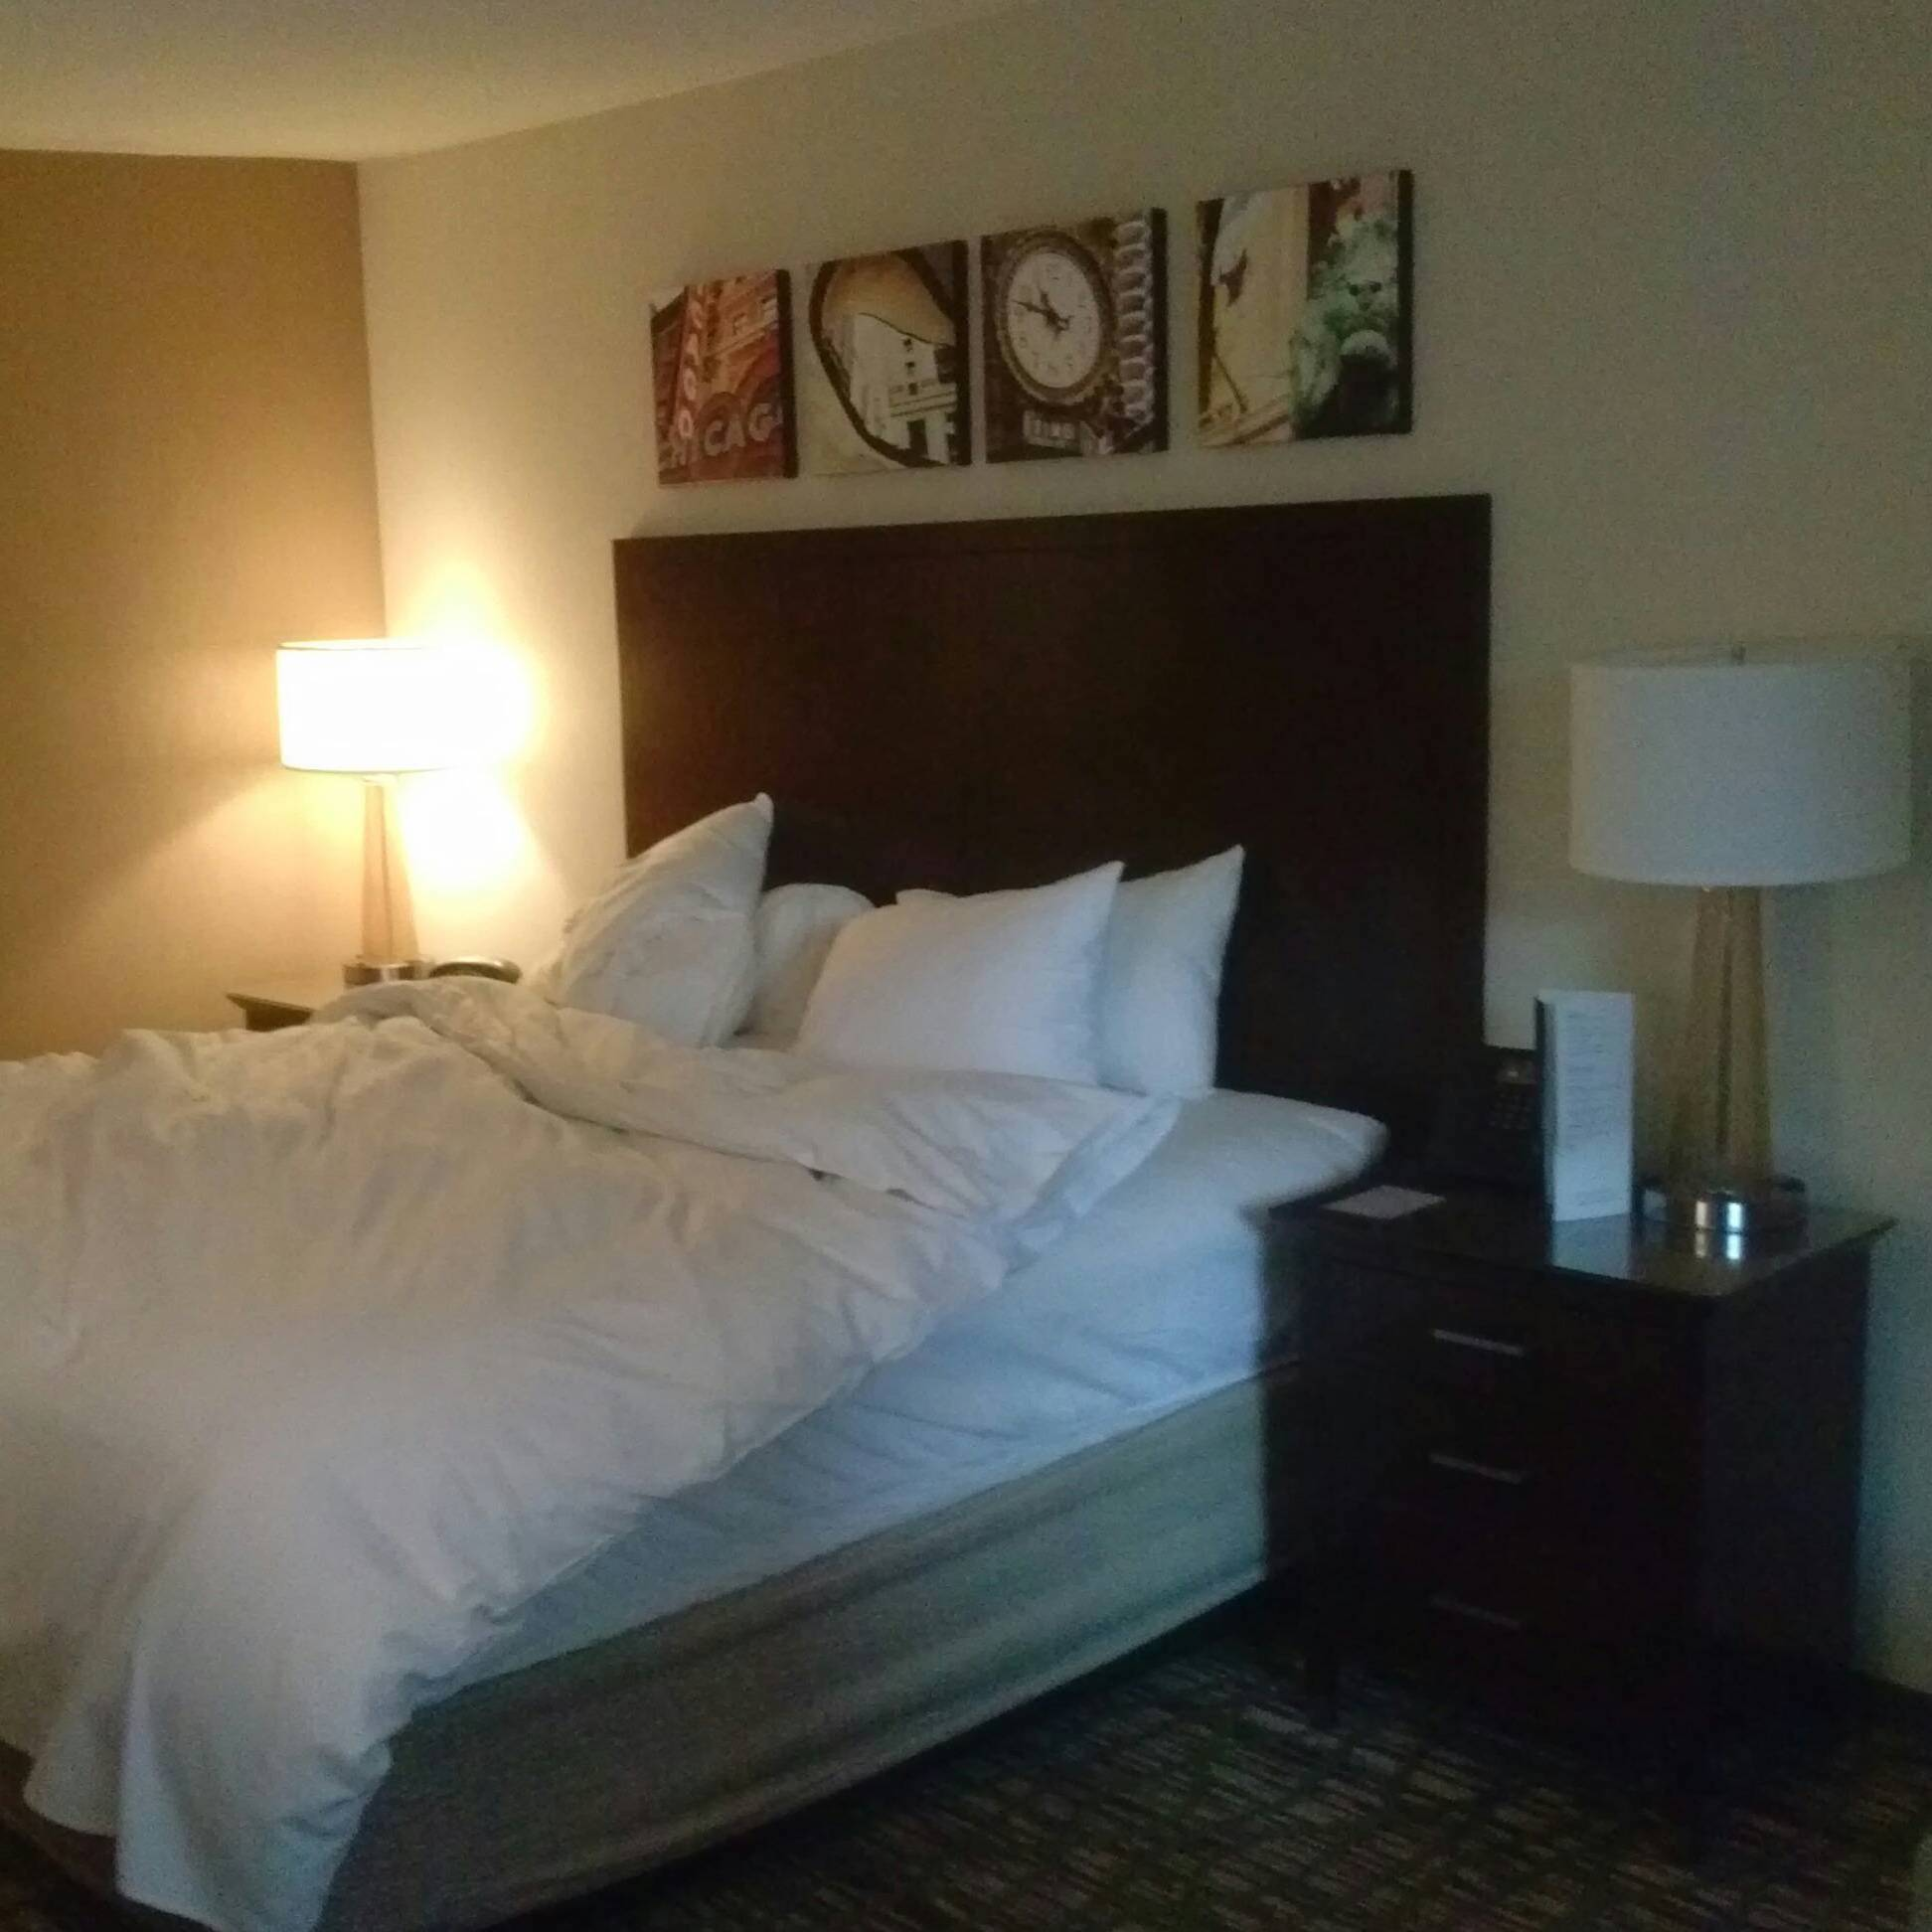
\includegraphics[width=.85in]{figs/exampleSearch/3}
            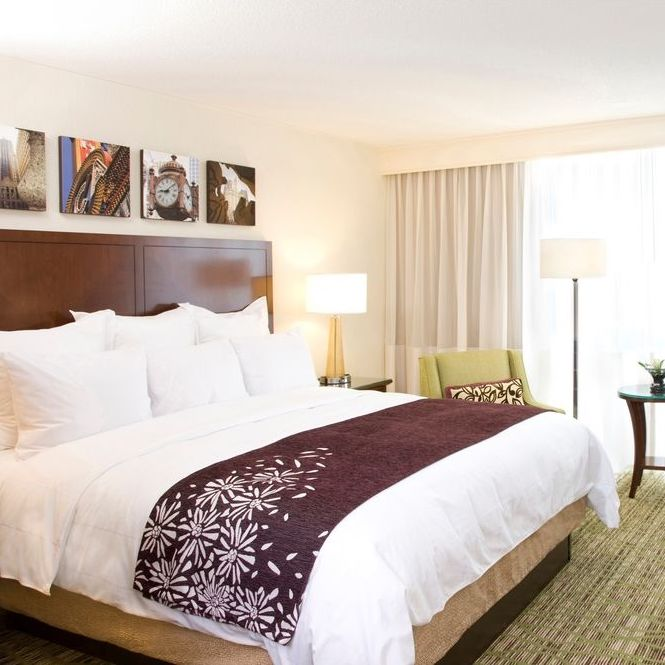
\includegraphics[width=.85in]{figs/exampleSearch/4}
            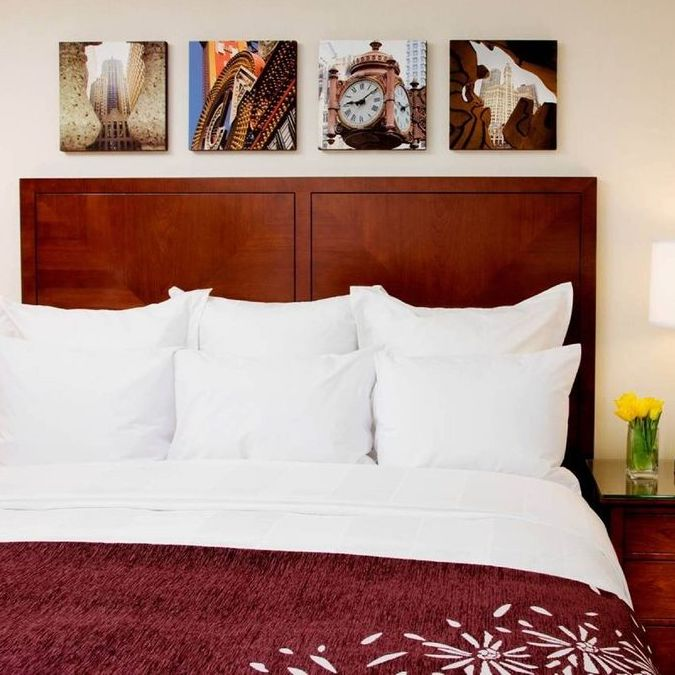
\includegraphics[width=.85in]{figs/exampleSearch/5}
            \caption{Closest matching images from TraffickCam}
            \label{fig:tcamResults_tCam}
        \end{subfigure}\\
        \begin{subfigure}[b]{4.4in}
            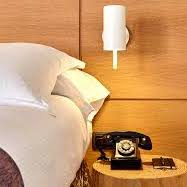
\includegraphics[width=.85in]{figs/exampleSearch/google1}
            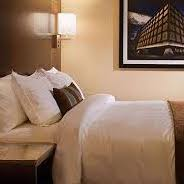
\includegraphics[width=.85in]{figs/exampleSearch/google2}
            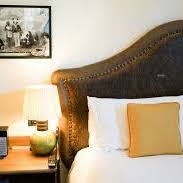
\includegraphics[width=.85in]{figs/exampleSearch/google3}
            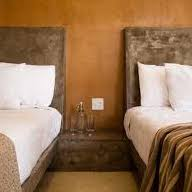
\includegraphics[width=.85in]{figs/exampleSearch/google4}
            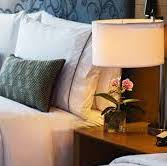
\includegraphics[width=.85in]{figs/exampleSearch/google5}
            \caption{Closest matching images in Google Image Search}
            \label{fig:tcamResults_google}
        \end{subfigure}
     \end{subfigure}
    \caption[TraffickCam vs. Google Image Search]{Comparison of the top image matches from TraffickCam and Google Image Search. The query was known to be from a Chicago Marriott hotel. The top five results from TraffickCam are from the exact hotel or another Marriott hotel. Google Image Search provides unrelated results, likely due to the large occlusion from the victim in the photograph.}
    \label{fig:tcamResults}
\end{figure}

\begin{figure}
    \centering
    \begin{subfigure}[b]{3.1in}
        
\includegraphics[width=3in]{figs/europol/twitter}
        \caption{}
        \label{fig:europolTwitter}
    \end{subfigure}
    \unskip \hspace{0pt}
    \begin{subfigure}[b]{3.1in}
        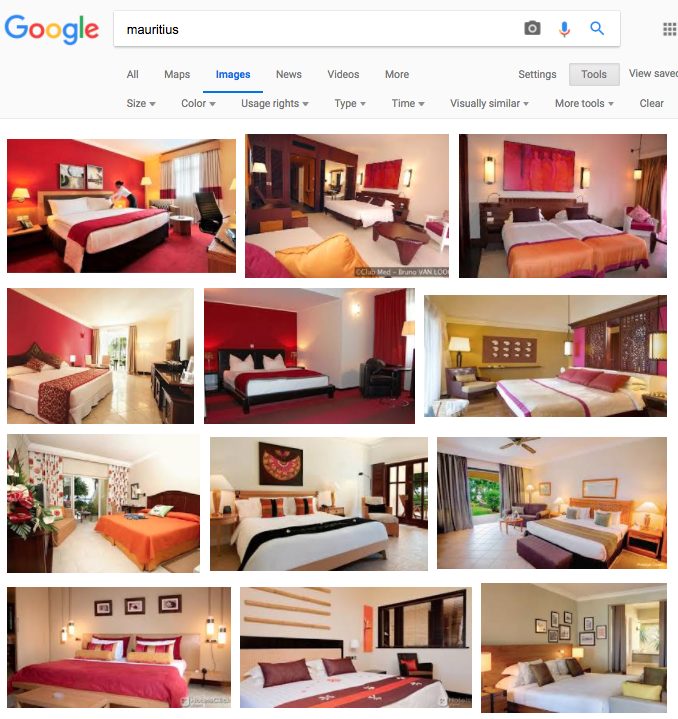
\includegraphics[width=3in]{figs/europol/google}
        \caption{}
        \label{fig:europolGoogle}
    \end{subfigure}\\
    \begin{subfigure}[b]{3.1in}
        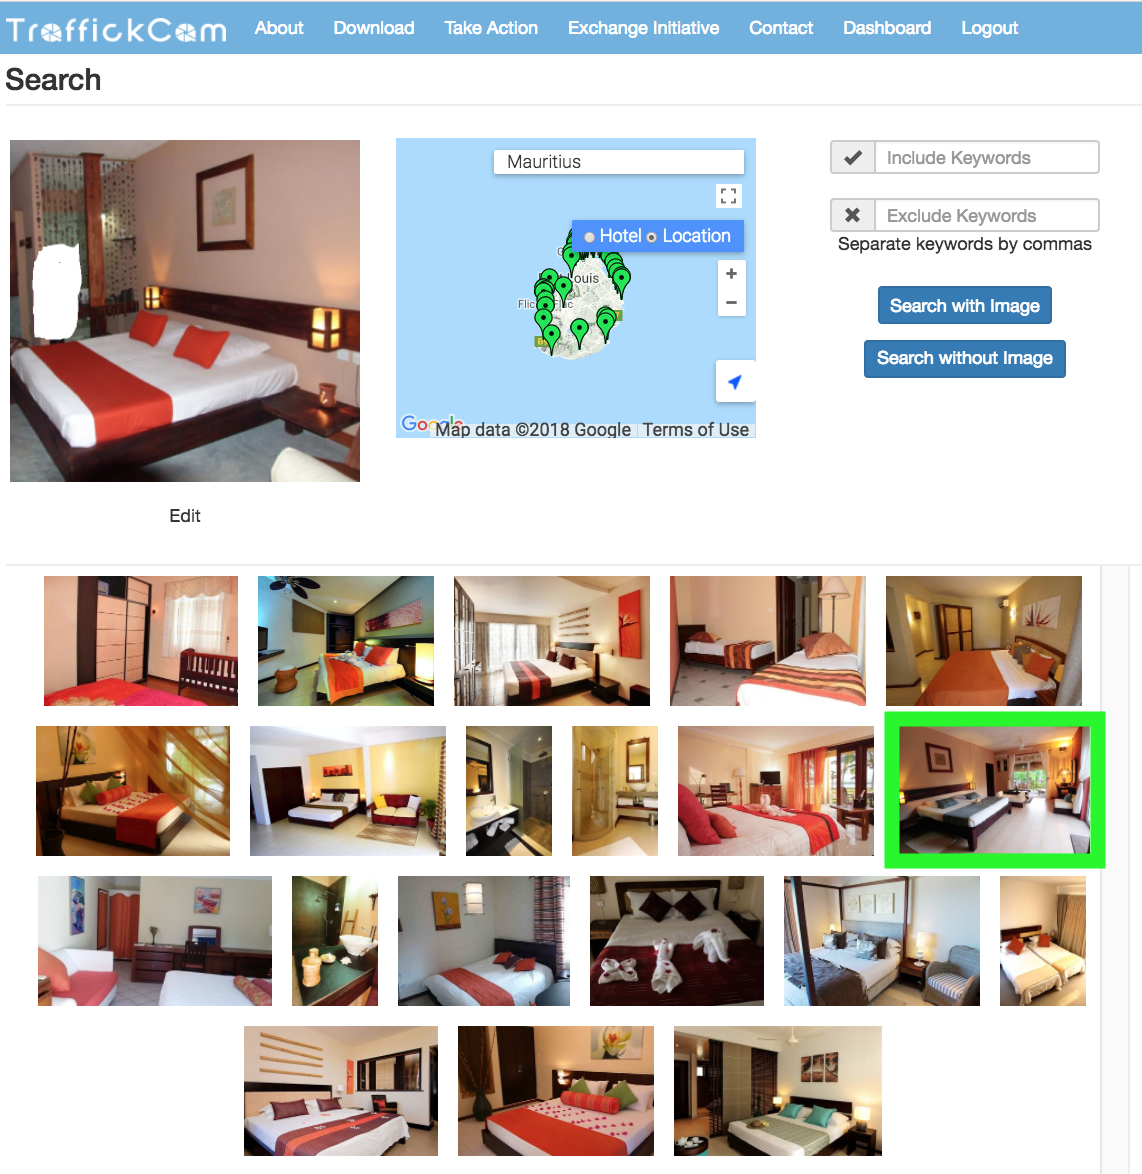
\includegraphics[width=3in]{figs/europol/tCam}
        \caption{}
        \label{fig:europolTcam}
    \end{subfigure}
    \unskip \hspace{0pt}
    \begin{subfigure}[b]{3.1in}
        \raisebox{.6in}{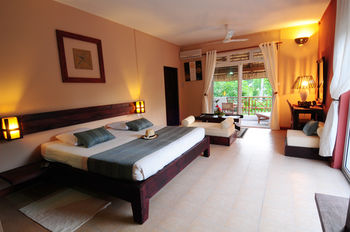
\includegraphics[width=3in]{figs/europol/correctResult}}
        \caption{}
        \label{fig:europolCorrectResult}
    \end{subfigure}
    \caption[Example results on Europol image challenge]{(a) Europol challenge to help identify the hotel location in victim photograph. (b) Google Image Search results, all of which focus on the color profile from the query image. (c) TraffickCam results, including a match to the correct hotel labeled in green and shown in (d). Note that this result is from a different view and contains different colored linens.}
    \label{fig:europol}
\end{figure}

In another demonstration, we applied TraffickCam to a public request for assistance from Europol on August 11, 2017, where the task was to determine the hotel where a photograph of child victims of sexual abuse had been taken. Figure~\ref{fig:europol} shows a comparison of TraffickCam and Google Image Search on this task. Even when the country of interest (Mauritius) was included as part of the search, none of the most visually similar results from Google Image Search are from the same hotel. By comparison, the eleventh result from TraffickCam matches the correct hotel. Part of the challenge with this particular query image was that none of the online photographs from this hotel have the same color bed linens as the victim photo. The Google Image Search results appear to predominately focus on visual similarity to the bright orange linens in the victim photograph. On the other hand, TraffickCam has been trained to match hotel rooms with different colored linens and can return matches with other visually similar characteristics. 

While TraffickCam currently outperforms general-purpose image similarity tools for the task of matching the hotel room from which an image was captured, we believe there are some design, development, and research questions that must be addressed in order to provide a more effective image search tool to human trafficking investigators that aligns with existing investigative methods.

\section{Proposed Research}

The following sections describe my proposed research work to address the research gaps and opportunities described in Section~\ref{sec:gaps}. These gaps currently impede the success of an AI-driven approach to image-based search which supports investigations focused on locating where photographs of victims of human trafficking were taken. The facets of this proposed approach are driven by the needs of the human trafficking investigators, specifically by allowing investigators to focus on objects of interest in the scene and to see visualizations that explain why the computer vision system returned an image or hotel as a good result.

%% Each section should follow the same template

% .0 Introduce Idea
% .1 Proposed Approach
% .2 Implementation and Evaluation
%       Include Awareness of potential pitfalls of proposed project design and feasibility of proposed actions to minimize and/or mitigate them.


\subsection{Object-Centric Image Analysis}
\label{sec:usability}

The current version of TraffickCam, like many modern computer vision algorithms, matches images to images. Often, the results of this image-to-image approach are plausible and the top matches correspond to images from hotels of the same chain; however, sometimes the results are of rooms from different hotels that have similar properties (e.g., similar paint colors and furniture shapes). In order to develop computer vision-based tools that more closely align with the investigative approach taken by law enforcement officers, and to return better hotel results, we describe an object-centric approach to image analysis. Moving from an image-centric to an object-centric approach requires changes to the both the underlying image representation and how images are collected and annotated.

\subsubsection{Proposed Approach}
\begin{figure}
    \centering
    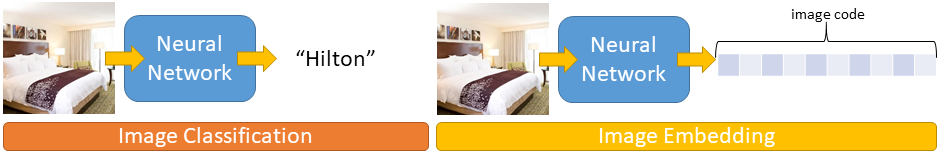
\includegraphics[width=.9\textwidth]{figs/classVsEmbed.png}
    \caption[Image embedding codes]{Unlike image classification, image embedding converts images to codes that can be used to support a variety of similarity-based image retrieval tasks.}
    \label{fig:embedding}
\end{figure}

Our proposed object-centric approach to image matching extends work in \emph{image embedding}, the task of mapping semantically related images to nearby points in some feature space. Figure~\ref{fig:embedding} compares image classification with image embedding. Image classification takes as input an image and outputs a classification (a hotel name, in our case). Image embedding converts an image to a code with the property that similar images should have similar codes. The results of a classification query are either right or wrong (e.g., the query photo either is or is not from a Hilton), whereas image embedding provides additional opportunities to analyze the results of a query. The distance from a query code to the database codes provides an indication of how close the query is to the different database images. In either case, similar machine learning models, including convolutional neural networks, can be used to learn the mapping from an input image to the desired output.

We propose to use \emph{structured embedding}, where we incorporate semantics into the coding learned by the model, in order to support an object-centric image search. In typical image embedding, a neural network will learn to return codes that are similar for images from the same hotel, but the codes themselves have no inherent meaning. In a structured embedding, a portion of the code can be used for that same purpose (i.e., matching images from the same hotel). Another portion of the code could be similar for images containing lamps, another for textured bedsheets, and so on. The neural network will be trained using multiple objectives so that a complex network of connections can be learned between images, objects, and hotels. Such an embedding would support the type of search where an investigator clicks on a particular object in the query image and receives results with similar objects based on the portion of the code corresponding to the object selected. This structured coding would allow for a similarity search where the results could be either based on whole image similarity, or additionally filtered by a specific object or even a more complex multi-object filtering (e.g., find images that have similar lamps \emph{and} similar artwork).  

\subsubsection{Implementation and Evaluation}

\begin{figure}
\centering
\begin{subfigure}[b]{3.5in}
\centering
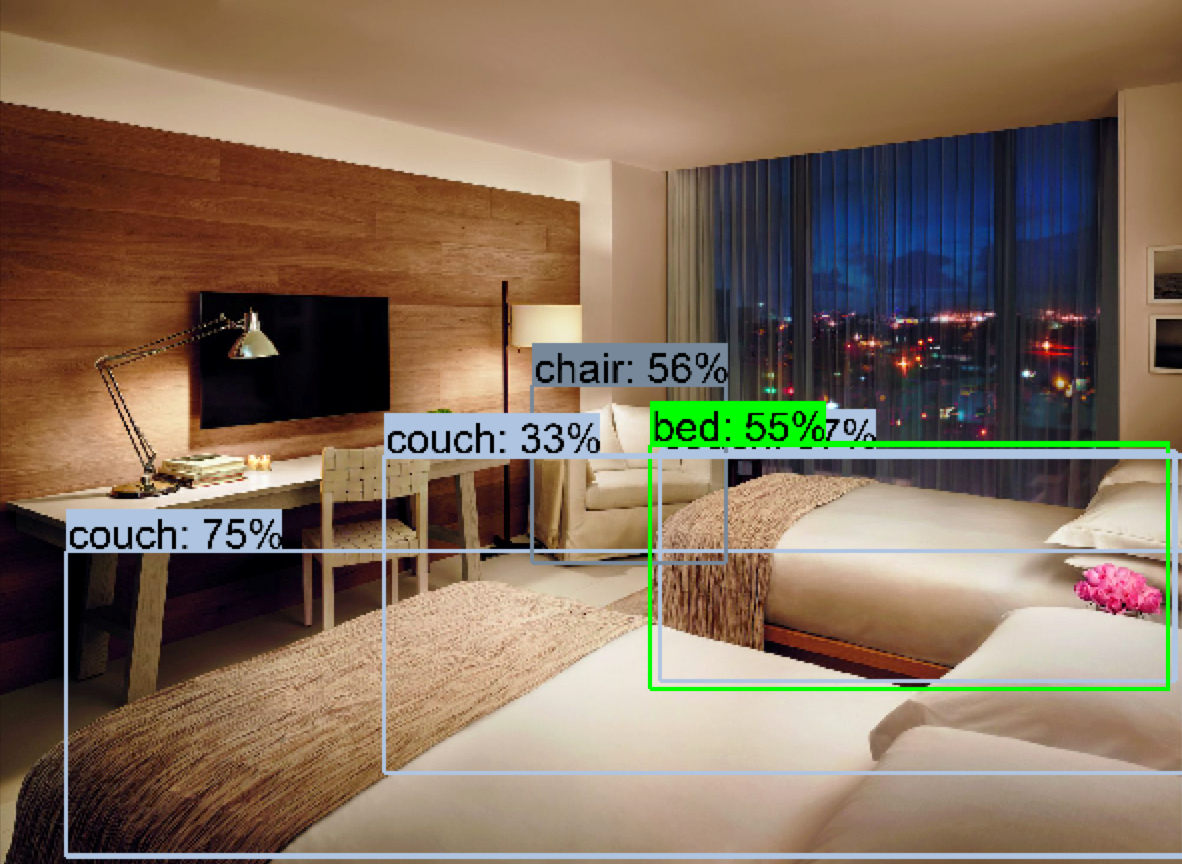
\includegraphics[height=1.4in]{figs/badObjects/example0.png}
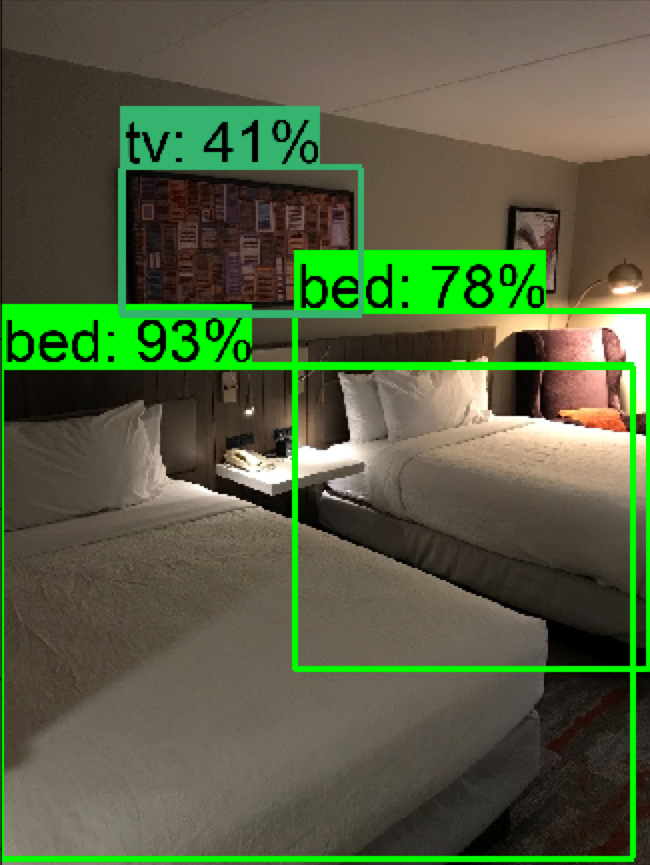
\includegraphics[height=1.4in]{figs/badObjects/example1.png}
\caption{Object detection on hotel room images.}
\label{fig:badObjects}
\end{subfigure}
\begin{subfigure}[b]{2.5in}
\centering
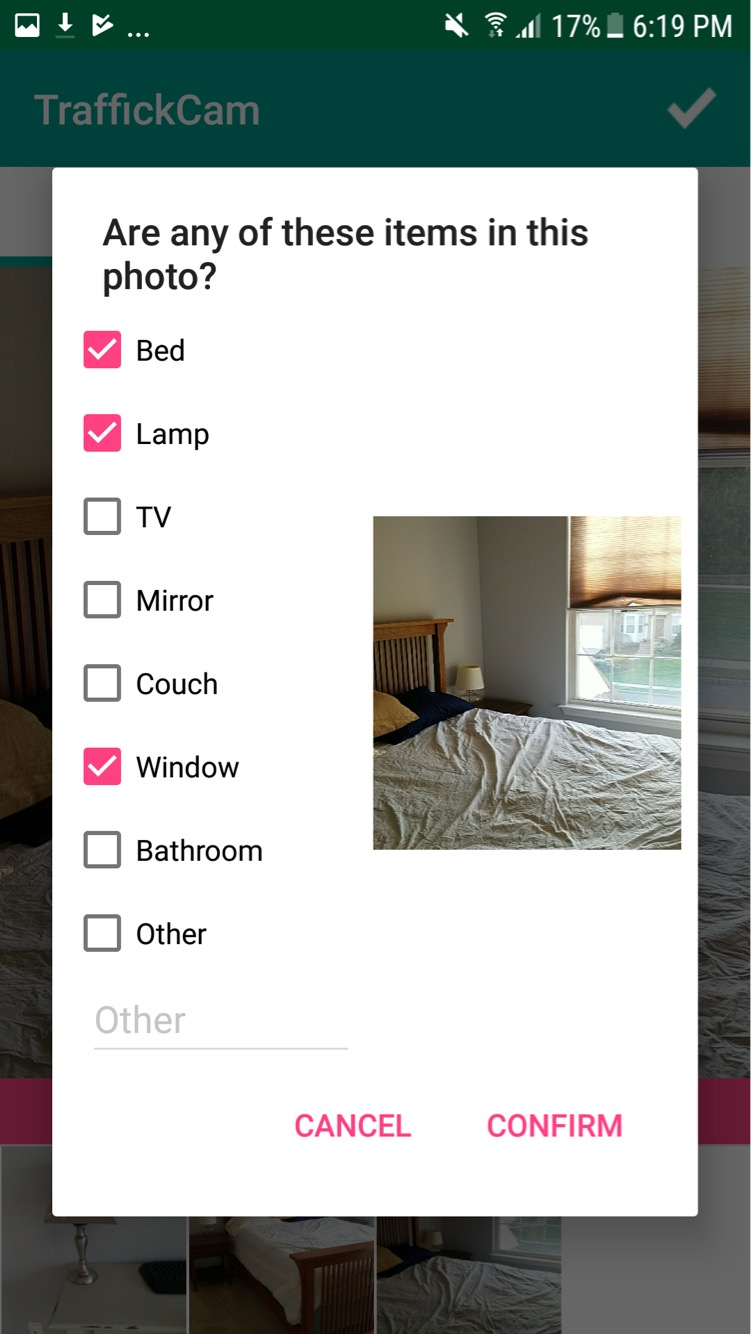
\includegraphics[height=1.4in]{figs/tCamVer2.jpg}
\caption{Object-centric mobile application.}
\label{fig:appVer2}
\end{subfigure}
\caption[Limitations of off-the-shelf object detectors]{Off-the-shelf object detectors do not always work well for identifying objects from hotel room images. We will develop a new version of our crowdsourcing application to collect object information with images.}
\label{fig:objectCentric2}
\end{figure}

Supporting object-centric analysis requires a large collection of images with annotated objects. In the field of computer vision, there is a long tradition of collecting and curating image sets. Some images sets such as ImageNet~\cite{imagenet_cvpr09},  
MSCOCO~\cite{DBLP:journals/corr/LinMBHPRDZ14}, and Scene Understanding (SUN)~\cite{xiao2010sun} contain millions of annotated images of people, objects, and scenes. These large datasets are used to train generic object detectors. However, off-the-shelf object detectors do not always work well for identifying objects from hotel room images. Figure~\ref{fig:badObjects} shows an example of a state of the art object detector~\cite{DBLP:journals/corr/LiuAESR15} applied to some of the crowdsourced TraffickCam images. In the first image, the detector hallucinated three couches and missed a bed, and in the second image, confused art for a TV. 

One way to improve the performance of such detectors is to re-train (or fine-tune) the models on the type of images that will be analyzed. For that, we need a large collection of annotated hotel room images. We plan to develop an upgraded version of our mobile application that asks users to identify objects in the images they capture for TraffickCam (Figure~\ref{fig:appVer2}). We are confident that our ever-growing user base will continue to upload images and also spend the additional effort to annotate the objects in the scene, because research shows that, specifically for mobile applications, contributing to a societal good is one of the strongest motivators for users to participate in crowdsourcing campaigns~\cite{DBLP:journals/tosn/RestucciaDP16}.

We will evaluate our object-centric search both quantitatively and qualitatively. Quantitatively, we will compare the retrieval performance for a set of input images captured from known hotels in terms of how well the top results match the hotel, chain, and geographic region of the query. For the object-centric mobile application, we will compare how many images are provided by users compared to the current version. Additionally, we will compare the performance of automated object detectors trained with and without the annotated crowdsourced images. This object-centric search will also be deployed to law enforcement using the TraffickCam image search and their feedback on its usefulness in their investigations will be incorporated in the ongoing development of the object-centric search.

\subsection{Visualizations for Understanding}
\label{sec:viz}
The current TraffickCam search system returns hotel results based on the similarity of the features extracted from a trained neural network. The reason two images are determined by the network to be similar is sometimes obvious (e.g., both images contain the same furniture and/or the same color bedspread), but other times it is not immediately clear why the network finds similarities between a query and database image. In this section, we describe the visualization approaches we will develop and incorporate into the TraffickCam platform that highlight why images are included in the search results. These visualizations will help end-users, typically not experts in AI, to better understand how the underlying algorithms work, and, over time, determine the best ways to use the software. In addition to providing the investigator insight as to why the network matched images, the visualizations will help the investigator ignore spurious results (e.g., similar but not exact artwork on the wall), and can be used as evidence of why a particular hotel location is part of an investigation.

\subsubsection{Proposed Approach}
\newlength{\mywidth}
\setlength{\mywidth}{.9in}

\begin{figure*}
    \centering
    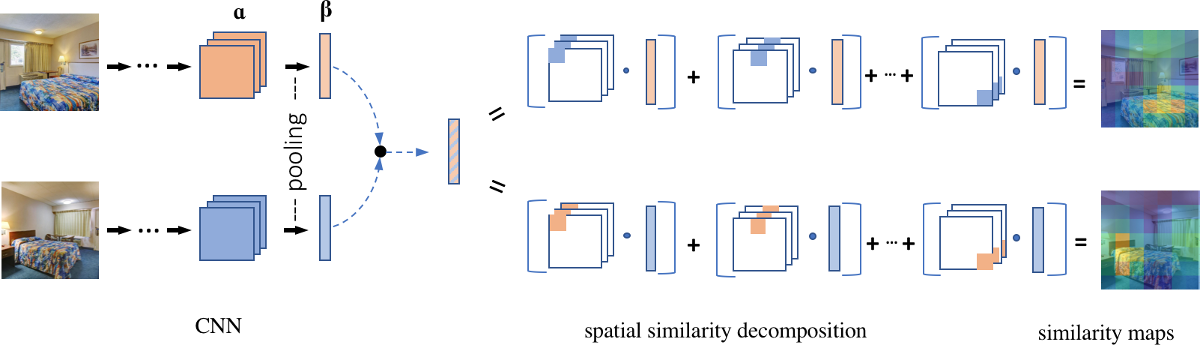
\includegraphics[width=0.9\textwidth]{figs/process.png}
    \caption[Proposed approach to visualizing similarity]{Our approach considers similarity networks with a final convolutional layer, $\boldsymbol{\alpha}$, followed by a pooling operation which produces output features, $\boldsymbol{\beta}$. Similarity between two images is measured as the dot product of these output features after normalization.  Factoring this value produces visualizations that highlight how much each region of the image contributes to the similarity.}
    \label{fig:visApproach}
\end{figure*}

The networks used in similarity learning broadly consist of: (1) a convolutional portion, (2) a ``flattening'' operation (usually max or global average pooling), and (3) a fully-connected portion, which is often used as the output feature on which similarity between pairs of images is computed. A recent study covering a number of image retrieval tasks, however, suggests that the best generalization performance is obtained using the output from the layer immediately after the pooling operation~\cite{vo2018generalization}. Rather than the traditional approach of computing a single value between these output feature vectors to measure similarity, we propose to analyze which which pixels in each image contributed to the activation of the corresponding components using the following approach.

Given an input image, $I$, and a trained similarity network, our approach to visualizing similarity relies on the activations of the layers before and after the pooling operation. Let $\boldsymbol{\alpha}$ be the $K \times K \times C$ tensor of the last convolutional layer, where $K$ represents the length and width and $C$ represents the number of filters. Let $\boldsymbol{\beta}$ be the $C$-dimensional vector after the pooling operation for an image, as shown in Figure~\ref{fig:visApproach}. In similarity learning, the dot product of these normalized feature vectors is a widely-used similarity function~\cite{bell2015learning,Proxy,schroff2015facenet,sun2014deep,wang2014learning,yi2014deep}, so the similarity of two images $I^{(i)},I^{(j)}$ can be written as:
\begin{equation}
s(\boldsymbol{\beta}^{(i)},\boldsymbol{\beta}^{(j)}) = \frac{\boldsymbol{\beta}^{(i)} \cdot \boldsymbol{\beta}^{(j)}}{\norm{\boldsymbol{\beta}^{(i)}} \norm{\boldsymbol{\beta}^{(j)}}}
\label{eq:cosineSim}
\end{equation}
Our visualization approach results in spatial similarity maps, where the overall similarity between two image feature vectors is spatially decomposed to highlight the contribution of image regions to the overall pairwise similarity, as shown in Figure~\ref{fig:visApproach}. Computing the similarity maps depends on the flattening operation between the convolutional portion of the network and the output feature.

For networks which employ average pooling as the flattening operation, the output feature, $\boldsymbol{\beta}$, is computed as:
\begin{equation} 
\boldsymbol{\beta} = \frac{1}{K^2}\sum_{x,y} \boldsymbol{\alpha}_{(x,y)}
\label{eq:avgPool}
\end{equation}
\noindent where $\boldsymbol{\alpha}_{(x,y)}$ represents the $C$-dimensional slice of $\boldsymbol{\alpha}$  at spatial location $(x,y)$. The similarity of images $I^{(i)}$ and $I^{(j)}$ can be directly decomposed spatially, by substituting $\boldsymbol{\beta}^{(i)}$ in Equation~\ref{eq:cosineSim} with Equation~\ref{eq:avgPool}:
\begin{align}
    s(\boldsymbol{\beta}^{(i)},\boldsymbol{\beta}^{(j)}) &= \frac{\boldsymbol{\beta}^{(i)}\cdot\boldsymbol{\beta}^{(j)}}{\norm{\boldsymbol{\beta}^{(i)}} \norm{\boldsymbol{\beta}^{(j)}}}\nonumber\\
    &=
    \frac{\frac{1}{K^2}\left(\boldsymbol{\alpha}^{(i)}_{(1,1)} + \ldots + \boldsymbol{\alpha}^{(i)}_{(K,K)}\right)  \cdot \boldsymbol{\beta^{(j)}}}{\norm{\boldsymbol{\beta}^{(i)}} \norm{\boldsymbol{\beta}^{(j)}}}\nonumber\\
    &= \frac{\boldsymbol{\alpha}^{(i)}_{(1,1)} \cdot \boldsymbol{\beta}^{(j)} + \ldots + \boldsymbol{\alpha}^{(i)}_{(K,K)} \cdot \boldsymbol{\beta}^{(j)}
    }{Z}
\end{align}
\noindent where $Z$ is the normalizing factor $K^2 \norm{\boldsymbol{\beta}^{(i)}} \norm{\boldsymbol{\beta}^{(j)}}$.

These terms can be rearranged spatially and visualized as a heat-map to show the relative contribution of each part of the image to the overall similarity. Symmetrically, the similarity can be decomposed to highlight the contribution of the other image in the pair to the overall similarity, as shown on the right side of Figure~\ref{fig:visApproach}.

\begin{figure}[t]
    \centering
    \begin{tabular}{cc}
        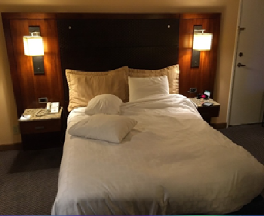
\includegraphics[width=.3\columnwidth]{figs/exampleVis/1_im.png} &  
        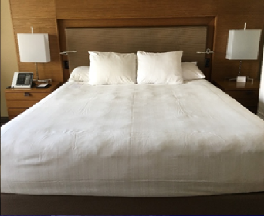
\includegraphics[width=.3\columnwidth]{figs/exampleVis/2_im.png}\\
        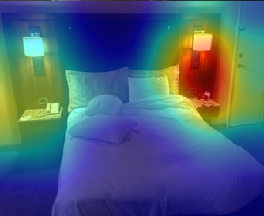
\includegraphics[width=.3\columnwidth]{figs/exampleVis/1_hm.png} &  
        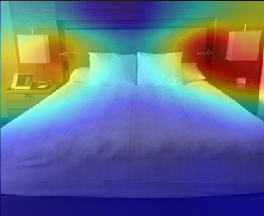
\includegraphics[width=.3\columnwidth]{figs/exampleVis/2_hm.png}
        \end{tabular}
    \caption[Example similarity visualizations]{(Top) Two images of rooms from different hotels whose output features resulted in high similarity scores. (Bottom) The visualization highlights the similar light fixtures mounted to the headboard, explaining why the network produced the high similarity score for a pair of images from different hotels.}
    \label{fig:exampleVis}
\end{figure}

We scale the heatmaps using bilinear interpolation and blend them with the original image to show which parts of the images contribute to the similarity scores. Figure~\ref{fig:exampleVis} shows an example of our visualization approach on a pair of TraffickCam images with a high similarity score. The visualization highlights that while the two images are actually from different hotels, the network produced high similarity scores for the pair of images because both rooms have similar light fixtures mounted to the headboard. This example demonstrates the ability of this visualization approach to explain why a network produces similar embeddings for a pair of images, even in cases where that may not be readily apparent to a human observer looking at the images.

% In our method for image embedding, a neural network is trained to convert images to a fixed length code, such that similar images have similar codes. In the case of TraffickCam, these codes are 128-dimensional vectors; the similarity between two images is computed as the dot product between the two 128-D vectors. The most similar result image to a query image is then the one that has the highest similarity score, or, the greatest number of very similar elements in their feature representations.

% There has been some work in computer vision and machine learning that shows that neural networks trained for classification and image embedding, like ours, decompose the task hierarchically and that some of the subtasks correspond well to object and region identification~\cite{scenecnn_iclr15}. That is, in the case of a network trained to match hotel room images, particulars neuron may correspond to whether or not there is a headboard in the scene, others for carpeting, others for artwork over a bed, etc. Rather than the traditional approach of computing a single value between a pair of feature vectors to measure similarity, we propose to analyze which \emph{components} of the two feature vectors are most similar and additionally compute which pixels in each image contributed to the activation of the corresponding components.

% Figure~\ref{fig:lampResults} shows two example visualizations where particular regions of each query image heavily contributed to the overall similarity score. In the first case, the relationship between the images is clear (i.e., similar lamps). However, in the second case, even though the top query matches come from the same hotel, the relationship between the highlighted regions is not as clear. By having an understanding of the objects in the scene, we can focus on those components of similarity that are most semantically meaningful to the end users. This approach allows us to generate visualizations by highlighting and color-coding regions of pixels from each image to explain semantic matches. 

% These visualizations can serve multiple purposes for human trafficking investigators using the TraffickCam system. In addition to providing explainabilty of the search results and underlying AI to an end user, and showing them why a particular query may have succeeded or failed, the visualizations can also be used as serve as method for the investigator to interactively provide feedback to the system. For example, if the visualization shows that the neural network is mapping two dissimilar objects or image components together, an investigator could click on a button to indicate a bad match. Such user-provided information could be incorporated during subsequent neural network training activities, improving the quality of future results.

% \begin{figure}
%     \centering
%     \begin{tabular}{c|ccccc}
%     Query & \multicolumn{5}{|c}{Best Database Matches} \\
%     \hline
%         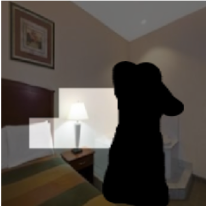
\includegraphics[width=\mywidth]{figs/lampSearch/query}  &
%         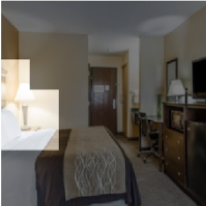
\includegraphics[width=\mywidth]{figs/lampSearch/1} &
%       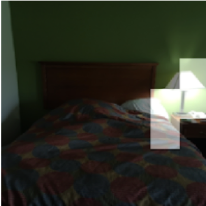
\includegraphics[width=\mywidth]{figs/lampSearch/2} &
%       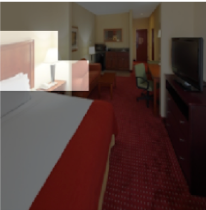
\includegraphics[width=\mywidth]{figs/lampSearch/3} &
%         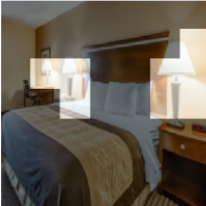
\includegraphics[width=\mywidth]{figs/lampSearch/4} &
%         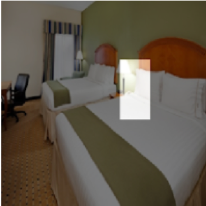
\includegraphics[width=\mywidth]{figs/lampSearch/5}\\
%     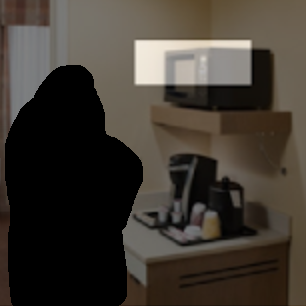
\includegraphics[width=\mywidth]{figs/embeddingViz/query}  &
%     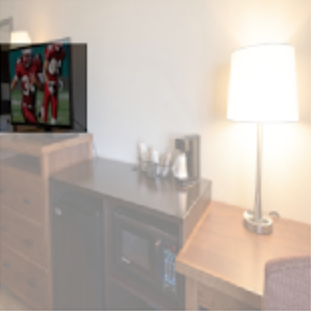
\includegraphics[width=\mywidth]{figs/embeddingViz/1}  &
%      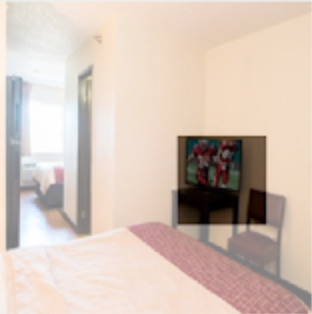
\includegraphics[width=\mywidth]{figs/embeddingViz/2}  &
%       \includegraphics[width=\mywidth]{figs/embeddingViz/3}  &
%       \includegraphics[width=\mywidth]{figs/embeddingViz/4}  &
%         \includegraphics[width=\mywidth]{figs/embeddingViz/5}  \\ 
%     \end{tabular}
      
%     \caption[Example visualization of matching image regions]{Example searches showing a query and the top matches with the image regions contributing the most to the similarity scores highlighted. In the first case, the images all contain similar looking lamps. In the second case, the relationship is not as clear.}
%     \label{fig:lampResults}
% \end{figure}

\subsubsection{Implementation and Evaluation}

The visualizations described above can be directly incorporate into TraffickCam search results. We also intend to explore alternative visualization approaches that incorporate the object-centric information described in Section~\ref{sec:usability}. For example, both the query image and resulting candidate images could be color-coded based on which specific objects in the images produced similar activations in the neural network (e.g., highlight in blue a similar looking lamp in both images, highlight in green a similar looking headboard), as opposed to the current approach which simply encodes any image locations that contribute highly the similarity score. We will provide an option in TraffickCam for users to select whether or not such visualizations are included as part of the search results, allowing us to assess the quality and utility of the visualizations in terms of how well it aids member of investigators in understanding the system and performing investigative tasks. 

\section{Impact of This Work}
Images of human trafficking victims are often shared by traffickers among criminal networks and posted in online advertisements. These images contain clues as to the location the image was captured. Our proposed search tools will be better able to link victims in images to particular places. This can serve to create links between different people seen in the same rooms, or many different hotel locations seen in different images. For instance, proving that a victim was moved across state lines may lead to additional or upgraded charges. This image search platform for law enforcement will support investigations to rescue and support trafficking victims, avoid their re-victimization, and to prosecute their traffickers to the fullest extent of the law. 

Since the initial deployment and popular press about TraffickCam~\cite{washingtonpost,techcrunch,cnn}, we have maintained a list of hundreds of law enforcement agencies that have requested information about and access to these search tools. This list not only highlights the need for such tools, but provides a path for the dissemination of the updated image search system based on the research performed in the remainder of my dissertation work to groups that are actively interested in using TraffickCam to investigate and prosecute human trafficking.

While the scope of this proposal has focused on human trafficking, it is the case that other illicit activities also occur in hotel rooms, for example, drug or weapons trafficking. The tools and algorithms developed in the course of this project could be applied to a broader set of cases. Additionally, the research ideas in this work, specifically on object-centric image similarity and visualizing why neural networks produce similar feature representations for images, extend beyond hotel rooms specifically, and have broader applicability to the AI, computer vision, and machine learning research communities.

\singlespacing
\bibliographystyle{abbrv}
\bibliography{refs,biblio}
\newpage
\pagenumbering{gobble} 

\end{document}